\def\OtherAuthors{ and (primarily) Jonah Sachs}
\SetTitle{40}{Variational Quantum Eigensolvers}{High-level introduction}{40}


\begin{frame}{Overview}{A brief introduction}
\begin{enumerate}
    \item Given a matrix (H), we wish to find the set of eigenvalues associated with H. VQE's goal is  finding the smallest eigenvalue of H, but it can be modified to also find higher-level eigenvalues
    \vspace{5mm}
    \item We can analytically find the eigenvalues of H through matrix decomposition methods. The issue arises when H becomes large enough that it can no longer be analytically solved.
    \vspace{5mm}
    \item As of 20 years ago, the largest classically solved matrix was through Google's PageRank algorithm. The generated eigenvector was 2.7 billion web pages long.
    
\end{enumerate}
\end{frame}

\begin{frame}{Brief Mathematical Recap} {Quantum Kickstart}

Eigenvalue Equation: $$H | \Psi \rangle = E_n |\Psi \rangle$$

\textbf{Definitions}
\begin{enumerate}
    \item H - the Hamiltonian Matrix. In physics, this represents the total energy: \( H = KE + PE \), where \( KE \) is the kinetic energy and \( PE \) is the potential energy. It can also represent optimization problems and other complex systems. 
    \vspace{2mm}
    \item \textbf{$| \psi \rangle$} - a State Vector in quantum mechanics, commonly referred to as a "ket". It is a general eigenvector of the Hamiltonian Matrix. 
    \vspace{2mm}
    \item $E_n$ - A discrete energy level of the system represented by H. In mathematical terms, this is the eigenvalues of H. In VQE, we are searching for $E_0$, the minimum energy level
    \vspace{2mm}
    \item $| x \rangle$ - a state vector of the computational basis. For 1 qubit, $| 0 \rangle$ and $| 1 \rangle$.
\end{enumerate}

\end{frame}

\begin{frame}{VQE Pipeline}{How the algorithm actually works}

The Steps of VQE given step by step:
\vspace{2mm}
\begin{enumerate}
    \item Hamiltonian Construction 
    \item Encoding of the Operators (Hamiltonian Deconstruction)
    \item Ansatz and State Preparation (Expectation Value)
    \item Parameter Optimization
\end{enumerate}

\end{frame}

\begin{frame}{VQE Pipeline}{An Overview}


\vspace{2mm}
\begin{enumerate}
    \item \ColorB{Hamiltonian Construction}
    \item \ColorB{Encoding of the Operators (Hamiltonian Deconstruction)}
    \item \ColorG{Ansatz and State Preparation (Expectation Value)}
    \item \ColorB{Parameter Optimization}
\end{enumerate}
\vspace{5mm}
The \ColorB{blue} steps are done either using a classical computer or analytical methods

\vspace{5mm}
The \ColorG{green} step is done using a quantum computer

\end{frame}


\begin{frame}{Hamiltonian Assumptions}{Why is this faster anyway?}
\vspace{-2mm}
\begin{enumerate}
    \item So we're only calculating expectation values on the quantum computer. Why should we care about VQE at all?
    \item In the long term, Quantum Computers will offer speedup for full analytical solutions of Hamiltonian matrices (FQE), but this will require millions of physical qubits for actualization 
    \item The speedup of VQE comes from the decomposition of the Hamiltonian matrix
    % \item VQE is a compromise between quantum speedup and error induced by NISQ systems.
    \item For VQE, we will assume the complex Hamiltonian is actualized and defined by the system (Step 1)
    \item For any complex Hamiltonian, we also assume it can be decomposed into the addition of Pauli Strings $(P_i \TensOp P_i \TensOp ... \TensOp P_i) \quad P_i \in \{X,Y,Z,I\}$ (Step 2)
    \item For a NxN matrix, we will have at most O(Poly(N)) Pauli Strings for an NxN Hamiltonian.
    \item The length of the Pauli Strings determines the number of qubits required for VQE
    
\end{enumerate}
\end{frame}


\begin{frame}{Measuring with the Hamiltonian- Pauli Gate Tricks}{On a Quantum Computer}
\vspace{1mm}
 \begin{itemize}
     \item We wish to measure in the Z basis to receive results akin to $| x \rangle$
     \vspace{2mm}
     \item  We can rotate results in the other bases to perform measurements in the Z axis.
     \vspace{2mm}
     \item The gates listed below indicate how we rotate the results of each Pauli operation back into the Z basis.
 \end{itemize}



 
\TwoColumns{%
\begin{center}
$ \PauliX : \Hadamard $ Hadamard
\vspace{2mm}

$ \PauliY : R_x (\frac{\pi}{2}) $
\vspace{2mm}

$ \PauliZ: \text{no rotation} $
\vspace{2mm}

$ \Identity: \text{ no measurement performed}$
\end{center}
}
{%
\vspace{-3mm}

 *note expectation values of the Pauli operators map a measurement of \QZero \hspace{0.5mm} to 1 and \QOne \hspace{0.5mm} to -1 due to the eigenvalues of the Pauli \textbf{Z} gate.

 \vspace{4mm}
 *note also that \textbf{I} can be ignored since the result will always be constant. We can add back this offset manually
}
\end{frame}

\begin{frame}{Pauli Strings}{Representation and Measurement}
\begin{itemize}
    \item More complicated Hamiltonians can exist with combinations of multiple Pauli gates on a singular qubit
    \item  Relationships between the Pauli gates can be used to simplify these complex expressions.
    \item Ignoring phase, more complex expressions can often be simplified into a singular Pauli gate.
\end{itemize}

\TwoColumns{% 
\vspace{3mm}
\begin{center}
\begin{tabular}{|c | c c c|} 
 \hline
 multiply & \PauliX & \PauliY & \PauliZ \\ [0.5ex] 
 \hline
 \PauliX & \Identity & i\PauliZ & -i\PauliY \\ 
 \PauliY & -i\PauliZ & \Identity & i\PauliX \\
 \PauliZ & i\PauliY & -i\PauliX & \Identity \\
 \hline
\end{tabular}\
\end{center}
}
{%
\vspace{-8mm}
\begin{center}
For example take the Hamiltonian for a single qubit:
$$ H = \alpha_1 \PauliX \PauliX + \alpha_2 \PauliY \PauliZ + \alpha_3 \Identity \PauliZ $$
This can be simplified to the following where i is just a phase factor and can be ignored:
$ H = \alpha_1 \Identity - \alpha_2 i\PauliX + \alpha_3\PauliZ $
\end{center}
}
\end{frame}

\begin{frame}{Tricks we'll use!}{}
Listed below are mathematical tricks that will be utilized later:

\vspace{8mm}


    \begin{itemize}

        \item Generalized State Vector: $| \psi \rangle = \sum_{x}{\alpha_x  | x\rangle}$ 
        \vspace{2mm}
        \item  Selection Vector: $\langle x | \psi \rangle =  \langle x | \sum_{y} \alpha_{y} | y \rangle = \sum_{y} \langle x | y \rangle = \alpha_x \langle x | x \rangle = \alpha_x$ 
        \vspace{2mm}
        \item Probabilistic Interpretation: $P(|x\rangle) = |\alpha_x|^2 = |\langle x | \psi \rangle | ^2$
        \vspace{2mm}
        \item Classical Expectation Value: $E(x) = \sum_x xP(x)  $
        \vspace{2mm}
        \item  Quantum Expectation Value: $\langle H \rangle_\psi =  \langle \psi | H | \psi \rangle $
        
    \end{itemize}
        
   
   
\end{frame}

\begin{frame}{Expectation Values}{What did you expect?}
\begin{itemize}
    \item Below is a proof that our quantum expectation value formulation is equal to the classical definition
    \item Notice the classical definition is what we typically consider expectation value: $\sum (value)(P(value))$
\end{itemize}

\vspace{-7mm}
\begin{align*}
     \langle \psi | H | \psi \rangle \\
     &= \sum_{x,y} \alpha_y^* \alpha_x \langle y | H | x \rangle \\
     &= \sum_{x,y} \alpha_y^* \alpha_x E_n \langle y | x \rangle \\
     &= \sum_x \alpha_x^* \alpha_x E_n \\
     &= \sum |\alpha_x|^2 E_n \\
     &= E(E_n)
\end{align*}

\end{frame}




\begin{frame}{Variational Principle}{A Simple Bound}

\begin{itemize}
    \item Assume that $| \psi \rangle$ is no longer a general statevector, and instead a specific vector which we sample, $| \psi_n \rangle$. $| \psi_n \rangle$ is guaranteed to be an eigenvector of H
    \item All returned eigenvalues are guaranteed to be above the lowest eigenvalue in the spectrum, $E_0$, intuitively.
    \item Mathematically, we declare the effects of this as the variational principle:
    \begin{equation*}
        \langle H \rangle_{\Psi_n} = \langle \Psi_n | H | \Psi_n \rangle = E_n \langle \Psi_n | \Psi_n \rangle \geq E_0 \langle \Psi_n | \Psi_n \rangle 
    \end{equation*}
    \item We are seeking the minimum value of $E_0$ by calculating expectation values. But how do we vary our expectation value?
\end{itemize}

\end{frame}




\begin{frame}{A Variable $ |\psi \rangle$}{The Ansatz}
\begin{itemize}
    \item Visualize our vector $| \psi \rangle$ as a generic point on the tensor product of multiple Bloch Spheres
    \item There is a point, or specific vector $| \psi_n \rangle$, which achieves our minimum eigenvalue $E_0$
    \item Our goal is parameterizing a given  $| \psi_n \rangle$ to achieve that minimum point
    \item An example would be $U^{\TensOp n}$, which could reach every point in our vector space.
    \item This variable statevector is called \textbf{The Ansatz}
    \item An ansatz which spans the whole vector space is preferred, but can lead to problem slowdown. Ansatz's which only cover specific regions can also be used if the type of solution is known.
\end{itemize}

\end{frame}


\begin{frame}{Steps for a Quantum Computer Scientist}
    \begin{itemize}
        \item Prepare a Hamiltonian which represents the system and decompose it into Pauli Strings
        \item Prepare a parameterized wavefunction with a set of parameters \textbf{x}
        \item Apply $| \psi_n \rangle$ and H to formulate an Expectation Value on a quantum computer. (See Qiskit Estimators). Rotation may be neccessary to get back into the Z basis.
        \item Store the resulting eigenvalue: $E_n$ and parameters: \textbf{x} in a classical dictionary 
        \item The classical optimizer will use \textbf{x} and $E_n$ to minimize the results of the expectation value. 
    \end{itemize}
\end{frame}

% \begin{frame}{A Toy Example}{}

% \begin{itemize}
%     \item $H = A = \frac{1}{2}(Z \TensOp I \TensOp X) - 3(I \TensOp Y \TensOp Y)$ \\ \vspace{3 mm}
%     \item$\langle A \rangle_{\psi} = \frac{1}{2}\langle \psi | (Z\TensOp I \TensOp X) | \psi \rangle - 3 \langle \psi | (I \TensOp Y \TensOp Y) | \psi \rangle$ \\ \vspace{3 mm}
%     \item For Term A (1st term): $(Z\TensOp I \TensOp X) | \psi_A \rangle = E_A | \psi_A \rangle$  \vspace{3 mm}
%     \begin{itemize}
%         \item $|\psi_A \rangle = | \psi_Z \rangle \TensOp | \psi_I \rangle \TensOp | \psi_X \rangle $ \vspace{3mm}
%         \item $E_A = E_Z * E_I * E_X$ \vspace{3 mm}
%         \item General: For any given Pauli String, a set of gates exists to transform our given Hamiltonian basis back into the computational Z basis. 
%         \item Given these change of basis operators, we can oscillate over possible state vectors to produce a valid eigenvalue for both the computational basis and our Hamiltonian basis.  
%     \end{itemize}
% \end{itemize}






% \vspace{3 mm}


    
% \end{frame}

% \begin{frame}{A Toy Example}
%     \begin{itemize}
%         \item 
%     \end{itemize}
% \end{frame}



\begin{frame}{A Simple Example}{Step 1 and 2 of the pipeline}
    Let's say that hypothetically, we have the simplest system imaginable. Even simpler than the hydrogen atom as even the Hamiltonian for just a proton and an electron is egregious. 
    \vspace{2mm}

    Step 1: Scientists figure out the Hamiltonian for this system looks like the following written in the Hamiltonian basis:

    $$ H = 3 \QZero \langle 0 | +  1 \QZero \langle 1 |$$

    Step 2: When written this way the Hamiltonian encodes easily to the Pauli basis:
    \vspace{2mm}

    \TwoColumns{%
    $ \QZero \langle 0 | = 1/2 (\Identity + \PauliZ)$
    
    $\QZero \langle 1 | = 1/2( \PauliX + i \PauliY)$
    
    $\QOne\langle 0 | = 1/2 (\Identity - \PauliZ)$
    
    $\QOne \langle 1 | = 1/2( \PauliX - i \PauliY)$
    }
    {%
    $$H = 1.5\Identity + 1.5\PauliZ + 0.5 \PauliX + 0.5i\PauliY$$
    }
\end{frame}

\begin{frame}{Continuing the Simple Example}{Preparing the Ansatz}
\begin{itemize}
    \item Our Ansatz: $ | \psi_n \rangle = R_y(\theta) | 0 \rangle$ (simple but could not span all possible solutions)
    \item Our parameter to be optimized (\textbf{x}): $\theta$
    \item  Hamiltonian: $H = 1.5\Identity + 1.5\PauliZ + 0.5 \PauliX + 0.5i\PauliY$
    \item We assume the expectation value will be approximated over a certain number of measurements of the prepared circuit. We will take 100 shots for estimation. 
    \item We prepare 300 circuits. 100 with only our Ansatz to represent $\PauliZ$  in our Hamiltonian. 100 with our Ansatz and a Hadamard to represent $\PauliX$ in our Hamiltonian. 100 with our Ansatz and $R_x (\frac{\pi}{2})$ ($\PauliY$). \textbf{I}, the offset, can be ignored and can be added back later
    \item Each of these individual setups will apply the ansatz and then be rotated into the \textbf{Z} basis for measurement. Thus, each additive term is distinctly separated onto its own qubit.
\end{itemize}

\end{frame}


\begin{frame}{The Circuit for the Example}{visualizing the implementation}
\begin{itemize}
    \item Let's being with an initial guess of $\theta = \pi/2$.
    \item An example of what one of the prepared circuits may look as follows. Since our Hamiltonian only involves one qubit we can prepare the different measurements simultaneously:
\end{itemize} 



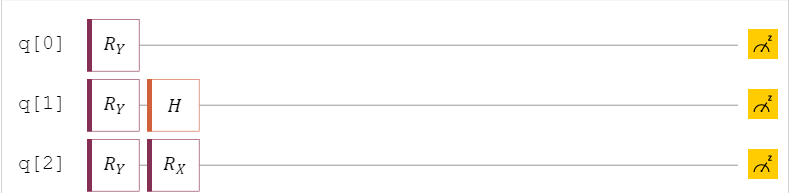
\includegraphics[scale = 0.5]{400/VQE_ex_circuit.PNG}

\begin{itemize}
    \item q[0] is our measurement in the $\PauliZ$ basis. q[1] is our measurement in the $\PauliX$ basis, and q[2] is our measurement is the $\PauliY$ basis.
    \item We prepare 100 of the above circuits.
    \item  Whenever we measure q[0] as $\QZero$ we add -1 to our calculation for the Hamiltonian expectation value in the $\PauliZ$ basis. If we measure $\QOne$ we add 1. 
\end{itemize}
\end{frame}

\begin{frame}{Finding the Expectation Value}{for the simple example}
We are solving 

$ \langle H \rangle_{\Psi(\frac{\pi}{2})} =1.5 \langle \Psi(\frac{\pi}{2}) | \Identity | \Psi(\frac{\pi}{2}) \rangle + 1.5 \langle \Psi(\frac{\pi}{2}) |  \PauliZ | \Psi(\frac{\pi}{2}) \rangle + 0.5 \langle \Psi(\frac{\pi}{2}) |  \PauliX| \Psi(\frac{\pi}{2}) \rangle $
 \vspace{4mm}
 
 $ + 0.5 \langle \Psi(\frac{\pi}{2}) |\PauliY| \Psi(\frac{\pi}{2}) \rangle$
 \vspace{1mm}

We do not need to perform any measurement for $Identity$. We assume it always returns the same value. The expectation value will be  one. 
 $\langle \Psi(\frac{\pi}{2}) | \Identity | \Psi(\frac{\pi}{2}) \rangle = 1 $
 \vspace{2mm}

For the $\PauliZ$ measurement 
 $\langle \Psi(\frac{\pi}{2}) |  \PauliZ | \Psi(\frac{\pi}{2}) \rangle = (1 + 1 -1 + 1... +1 -1) / 100 = \frac{-40 + 60}{100} = 0.2 $
 \vspace{2mm} 

For the $\PauliX$ measurement 
$\langle \Psi(\frac{\pi}{2}) |  \PauliX | \Psi(\frac{\pi}{2}) \rangle = (-1 - 1 -1 - 1... -1 -1) / 100 = \frac{-100}{100} = -1 $
\vspace{2mm}

For the $\PauliY$ measurement 
 $\langle \Psi(\frac{\pi}{2}) |  \PauliY | \Psi(\frac{\pi}{2}) \rangle = (1 + 1 -1 + 1... +1 -1) / 100 = \frac{-43 + 57}{100} = 0.14 $
\vspace{2mm}

\end{frame}

\begin{frame}{Finding the Expectation Value Cont.}

Now we just plug the measured values into the expectation value equation.
\vspace{2mm}

 $\langle H \rangle_{\Psi(\frac{\pi}{2})} =1.5*1+ 1.5*0.2 + 0.5*(-1) + 0.5*0.14$
 \vspace{2mm}

  $\langle H \rangle_{\Psi(\frac{\pi}{2})} =1.5+ 0.3 - 0.5 + 0.07 = 1.37$
 \vspace{2mm}

 We then store the expectation value of 1.37 with a $\theta$ value of $\pi/2$. This process will be repeated given a new guessed $\theta$ by the classical optimizer. The process described is for a singular function evaluation of the optimizer
    
\end{frame}



\begin{frame}{Example VQE Runs}

Notice that the energy is dipping below the minimum value. How is this possible?
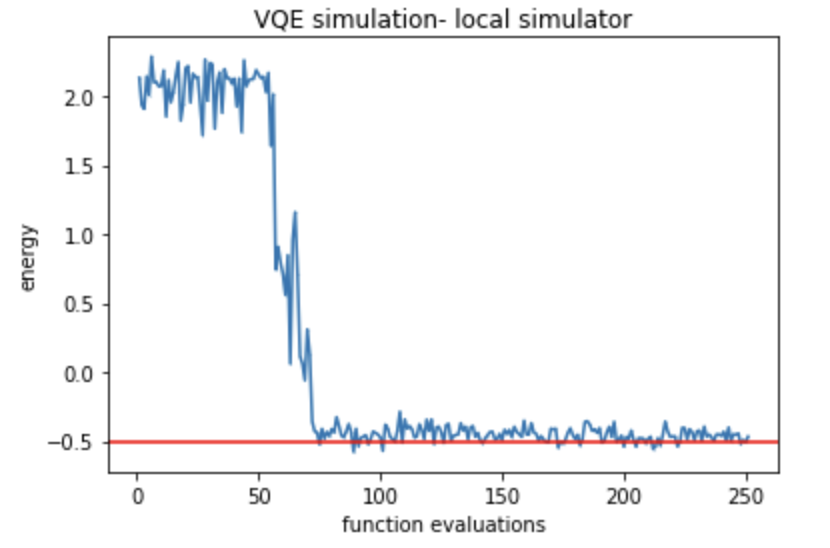
\includegraphics[scale = 0.3]{400/VQE_Ex_2.png}



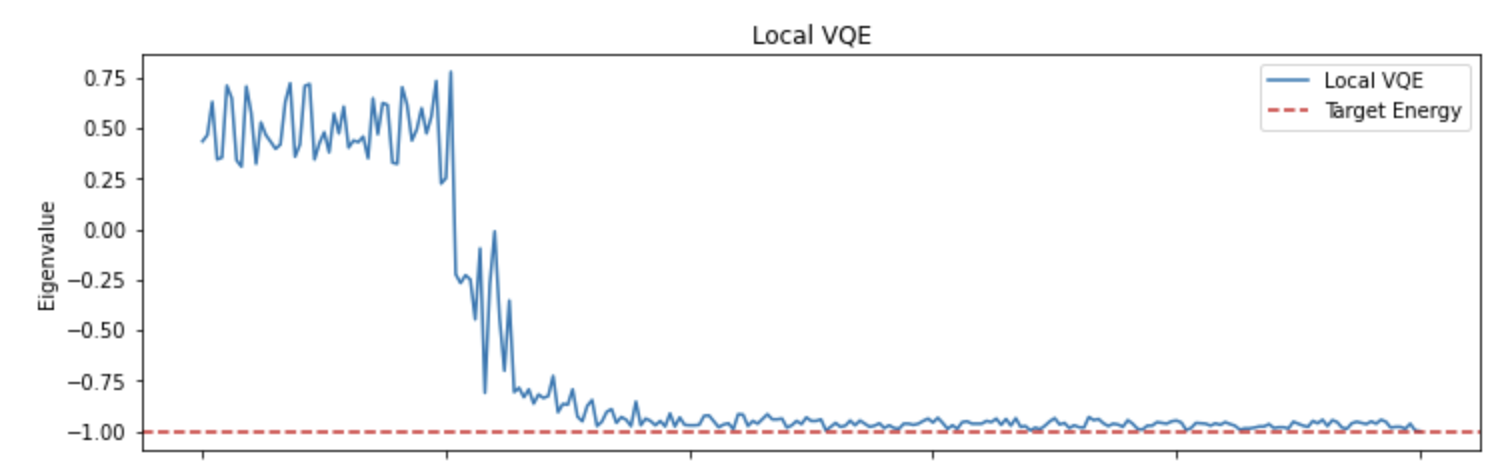
\includegraphics[scale = 0.35]{400/VQE_Ex_1.png}



\end{frame}

\begin{frame}{Optimization Changes}
    \begin{itemize}
        \item The optimizer used can  have a significant effect.
        \item SPSA uses gradient estimation, which causes the lack of convergence you see towards the target value. It can also causes overlap with the minimum value since estimations are made.
        \item A optimizer without gradient estimation will cause a cleaner result, but could more easily get stuck in local extrema. An example using COBYLA is given.
    \end{itemize}

    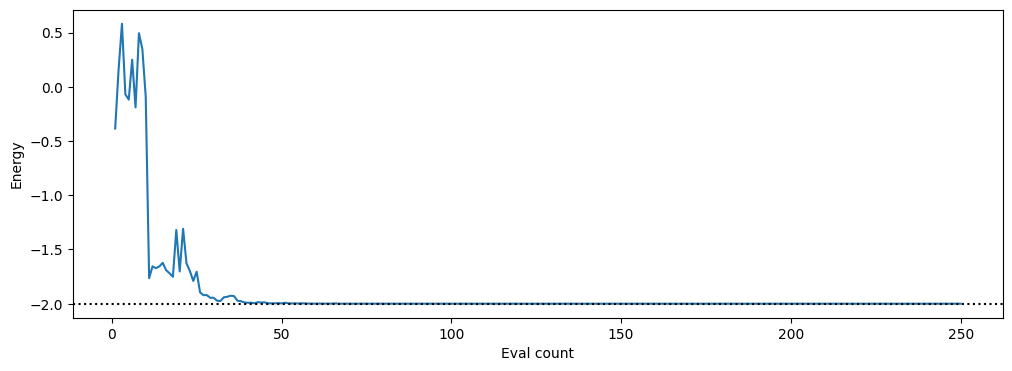
\includegraphics[scale = 0.35]{400/output.png}

\end{frame}

% \begin{frame}{Optimization Issues}

% The optimizers used for VQE are classical processes. Trials runs observed clear values below the ground state energy, which should not be possible due to the variational principle. Previously, we assumed the following definition of the Hamiltonian: $$H = \sum_i^{n} \alpha_i P_i$$.

% The typical variance relationship in quantum mechanics is: $$<(\Delta H)^2> = <H^2> - <H>^2$$

% Although the Hamiltonian can be decomposed into Pauli operators, its variance does not decompose as smoothly, causing an error factor to become present




% \end{frame}


% \begin{frame}{Hamiltonian Variance}

% $\langle H \rangle_{\Psi} = \alpha_1 \langle \Psi_n | P_1 | \Psi_n \rangle + \alpha_2 \langle \Psi_n |  P_2 | \Psi_n \rangle + ... + \alpha_n \langle \Psi_n |  P_n | \Psi_n \rangle$

% \vspace{2mm}

% $\langle H^2 \rangle_{\Psi} = \alpha_1^2 \langle \Psi_n | P_1^2 | \Psi_n \rangle + \alpha_2^2 \langle \Psi_n | P_2^2 | \Psi_n \rangle + ... + \alpha_n^2 \langle \Psi_n |  P_n^2 | \Psi_n \rangle$

% \vspace{4mm}

% The Hamiltonian, as an operator, has definite states. This means typically, $$<(\Delta H)^2> = 0$$

% It is clear that is not the case here, given our decomposition of $<H>$ and $<H^2>$. The terms will not cancel out, forming a nonzero variacnce relation. Since the Hamiltonian is not a determinate operator, similar to how we consider it in quantum mechanics, we cannot consider every measurement of energy to be purely definite. Some variability, or error, will exist. 

    
% \end{frame}

% \begin{frame}{Proposed Error}

% This is taken from a paper by Kandala, Mezzacapo, et al written in 2017 about using VQE for the modeling of small molecules and quantum magnets. Let S be the number of samples, T be the length of the Pauli Strings, and $h_{max}$ be the max weight. The variance can be defined: 

% $$Var[H] = \sum_\alpha^T h_\alpha^2<\Delta P_\alpha^2>$$

% $$\epsilon = \sqrt{\frac{Var[H]}{S}} \leq \sqrt{\frac{T|h_{max}|^2}{S}}$$

% With this error, although a value below the ground usually cannot be produced by the Hamiltonian, it possible to just break over the cusp. Different methods for Pauli decomposition and different optimizers can have different effects on this issue.
    
% \end{frame}



\begin{frame}{A CS Example: Max Cut}
    \begin{itemize}
        \item We will now consider a more classical computer science example and how it can be decomposed to solve via VQE
        \item We will consider a simple example of the Max Cut Problem
        \item We will be given a  graph with nodes and unweighted edges. This assumes all edge weights are equal to one. Our goal is to find a maximum cut of the graph
        \item A cut is a physically drawn divide which splits the nodes into two sets. 
        \item But how do we maximize a cut?
    \end{itemize}
\end{frame}

\begin{frame}{A Simple Graph for Max Cut}
    \begin{itemize}
        \item We will consider the following simple example with 3 nodes and two edges
    \end{itemize}
    \begin{figure}[h]
    \centering
    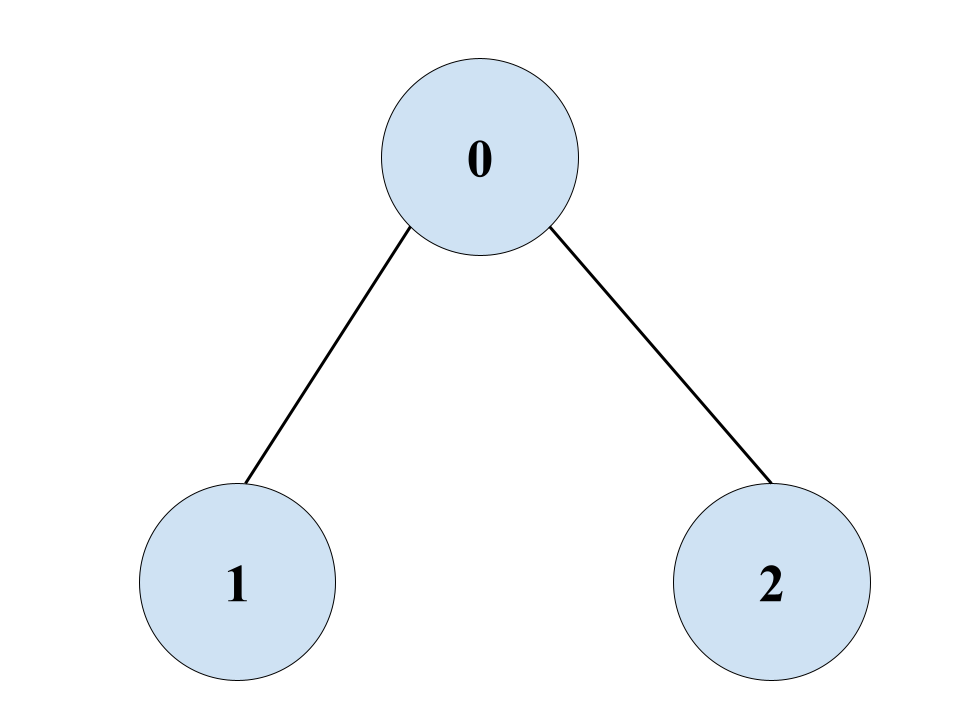
\includegraphics[width=0.6\textwidth]{400/Graph_MC.png}
    
\end{figure}
\end{frame}

\begin{frame}{An Example Cut}
    \begin{figure}[h]
    \centering
    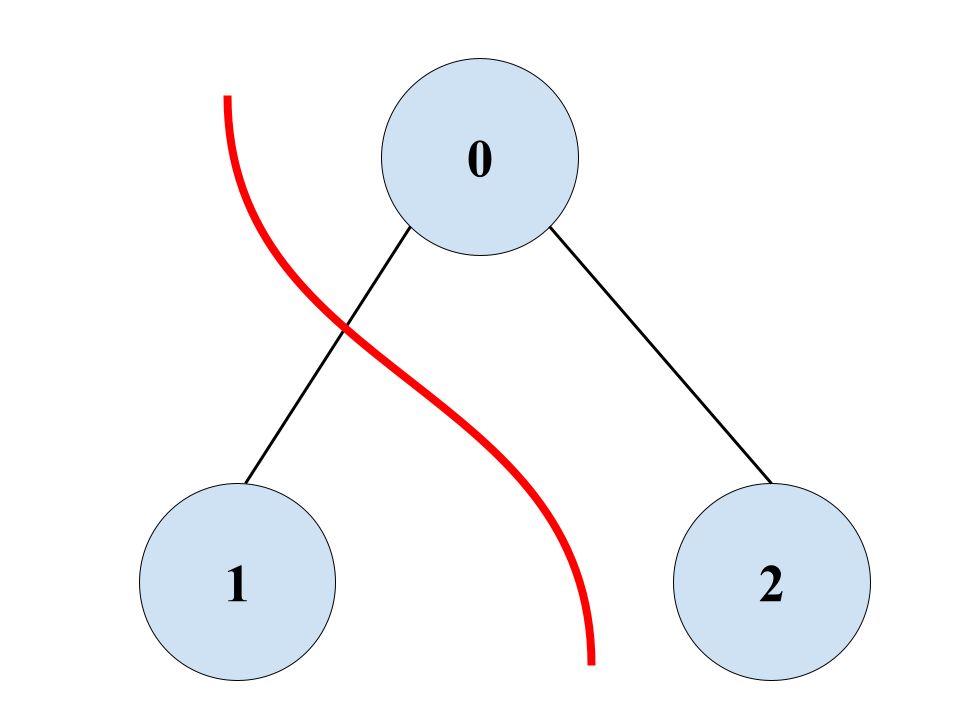
\includegraphics[width=0.4\textwidth]{400/Graph_MC_Cut.png}
    
\end{figure}
\begin{itemize}
        \item Lets propose an example cut 
        \item Our goal is to maximize the amount of broken edges that allow our nodes to be placed in two distinct sets. This is the maximum cut
        \item In this situation, 1 edge was broken.
        
    \end{itemize}

    
\end{frame}



\begin{frame}{An Example Cut}{The Math}
    \begin{figure}[h]
    \centering
    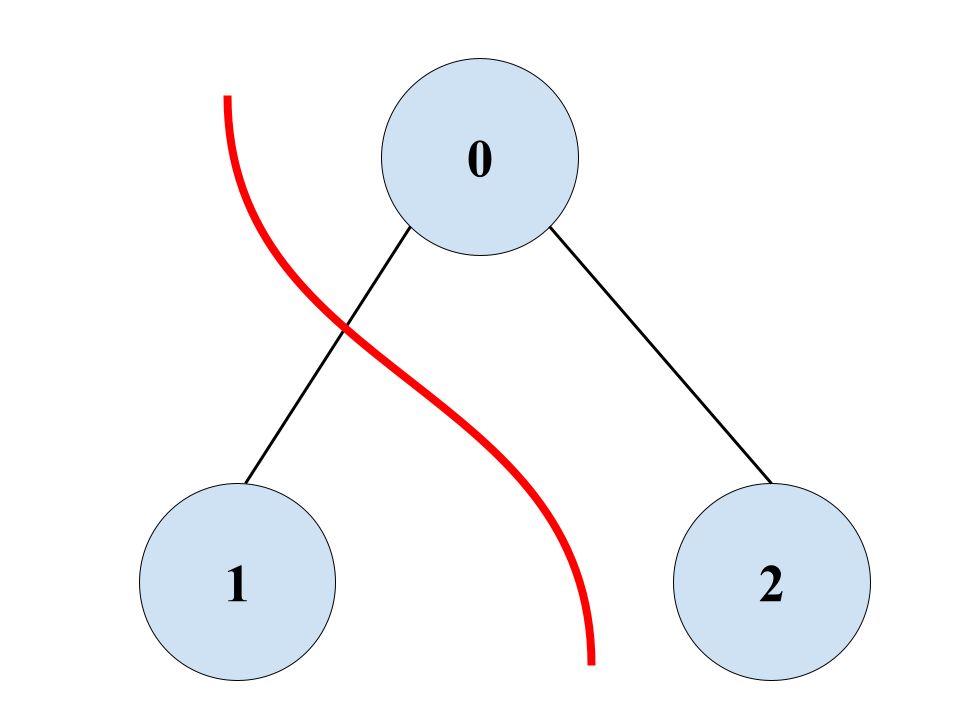
\includegraphics[width=0.4\textwidth]{400/Graph_MC_Cut.png}
    \end{figure}
    \vspace{-4mm}
    \begin{itemize}
    \item Let the value assigned to any node be represented by $z_i; z_i \in \{-1,1\}$
    \item The value of the node is assigned based upon which set the node is split into
    \item In this specific case: $z_1 = 1, z_0 = z_2 = -1$
    \item We notice the following: 
    \begin{itemize}
        \item For any two nodes in the same set $z_i z_j = 1$
        \item For any two nodes in different sets $z_i z_j = -1$ \textbf{When an Edge is Cut}
    \end{itemize}
\end{itemize}
\end{frame}

\begin{frame}{Maximizing the number of cuts}
    \begin{itemize}
        \item Thus, we return to our goal of maximizing the number of cut edges.
        \item Given the expression presented previously, we can iterate through all edges. Since all cut edges contribute a value of -1, our goal becomes minimization
        \item Mathematically, it can be defined as follows, where E  is the set of all Edges in the graph and j,k are node indices:
        \begin{equation}
            Minimize \sum_{(j,k) \in E} z_j z_k
        \end{equation}
        \item Above is the cost function of the system

        \item But how does Quantum Computing factor in? Do you remember the eigenvalues of the Pauli Z gate? 
        \begin{itemize}
            \item They are -1, 1! A measured Pauli Gate collapses to one of these eigenvalues (and corresponding eigenstate)
            \item Thus, we can cleverly use Pauli Z gates to represent every node variable $z_i$
        \end{itemize}
    \end{itemize}
    
\end{frame}

\begin{frame}{Quantum Decomposition}
\begin{itemize}
    \item Assume that every node of our graph receives a corresponding qubit. 
    \item Given equation (1) above, we convert to Pauli Gates.
    \item For our specific example, equation (1) translates to: 
    \begin{equation}
        min(z_0 z_1 + z_0 z_ 2)
    \end{equation}
    \item Assuming an identity for any qubit which does not experience a Z, this translates to the following.  
    \begin{equation}
        min(Z \TensOp Z \TensOp I + Z \TensOp I \TensOp Z) \quad 
    \end{equation}
    \item Later, this will be used as the Hamiltonian of the system.
\end{itemize}
    
\end{frame}

\begin{frame}{Brute Force Attack}{Complexity Nightmare}
    \begin{itemize}
        \item Lets consider the expectation value of all possible computational basis states of this 3-qubit system. This would not be possible for higher-dimensional systems.
        % \item The basis vector $|0\rangle$ maps to the eigenvalue 1 and $|1\rangle$ maps to -1. Thus, all basis vectors represent the nodes being placed into different sets. 
        \item Recall our quantum definition for the expectation value of a Hamiltonian H: $\langle \psi | H | \psi \rangle$
        \begin{center}
            \begin{tabular}{c|c|c|c}
                 $\psi$ & $\langle \psi | H | \psi \rangle$ & $\psi$ & $\langle \psi | H | \psi \rangle$ \\

                 $|000\rangle$ & 2 & $|100 \rangle$ & -2 \\
                 $|001\rangle$ & 0 & $|101 \rangle$ & 0 \\
                 $|010 \rangle$ & 0 & $|110\rangle$ & 0 \\
                 $|011\rangle$ & -2 & $|111\rangle$ & 2
            \end{tabular}
        \end{center}
        \vspace{2 mm}
        \item Notice that $|011\rangle$ and $|001\rangle$ achieve minima. What do these look like?
    \end{itemize}
\end{frame}

\begin{frame}{The Maximum Cut(s)}
    \begin{itemize}
        \item They are actually the same solution!
        \item Try drawing a ton of lines through the graph, is there more than one way to intersect both edges, while also splitting the nodes into two sets?
        \item The two solutions correspond to assigning each set to \{-1,1\}, but they are the same cut.
        \item The maximum cut is presented below:
        \begin{figure}[h]
    \centering
    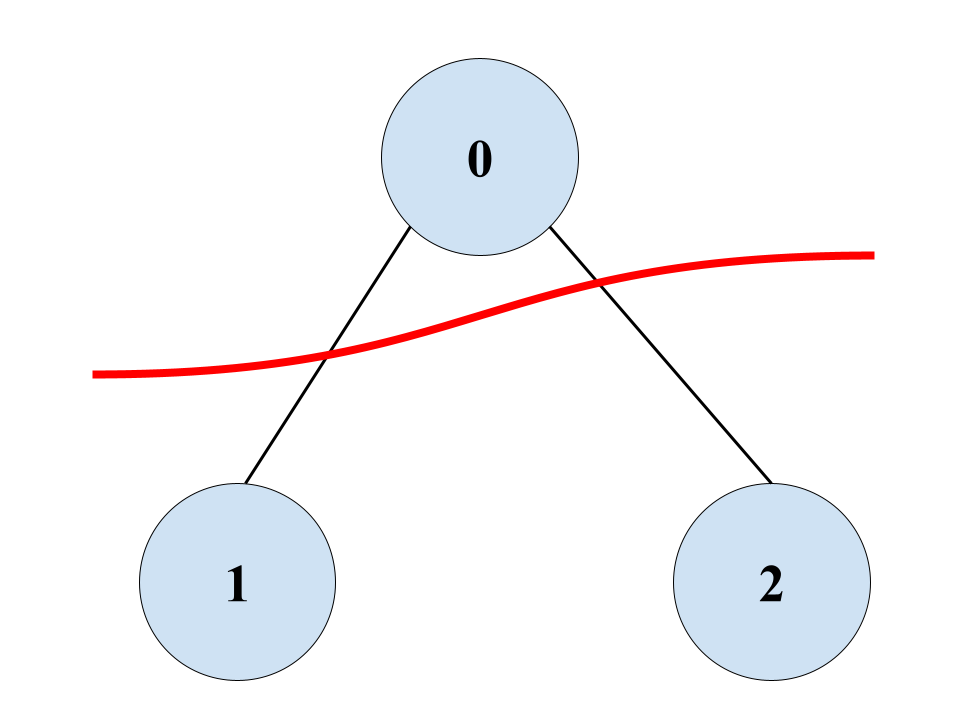
\includegraphics[width=0.4\textwidth]{400/Graph_MC_Cut_max.png}
    
\end{figure}
    \end{itemize}
\end{frame}


\begin{frame}{Back to Quantum}
    \begin{itemize}
        \item Does minimizing over expectation values sounds familiar? It should
        \item This is where VQE comes in. Given our produced Hamiltonian, we are still seeking the minimum eigenvalue. Now, we also wish to produce the eigenvector associated with it to analyze set declarations. Written analytically, the Hamiltonian is: 
    \end{itemize}
    \begin{equation}
        H \equiv \begin{bmatrix}
        2 & 0 & 0 & 0 & 0 & 0 & 0 & 0 \\
        0 & 0 & 0 & 0 & 0 & 0 & 0 & 0 \\
        0 & 0 & 0 & 0 & 0 & 0 & 0 & 0 \\
        0 & 0 & 0 & -2 & 0 & 0 & 0 & 0 \\
        0 & 0 & 0 & 0 & -2 & 0 & 0 & 0 \\
        0 & 0 & 0 & 0 & 0 & 0 & 0 & 0 \\
        0 & 0 & 0 & 0 & 0 & 0 & 0 & 0 \\
        0 & 0 & 0 & 0 & 0 & 0 & 0 & 2 \\
    \end{bmatrix}
    \end{equation}
    
\end{frame}


\begin{frame}{VQE Resources}
But we don't just need a Hamiltonian to perform VQE. Below I've described the other variables declared.
    \begin{itemize}
        \item \textbf{Ansatz}: The variable wavefunction. Has been declared as a combination of $R_y$ (rotation) and CNOT (entanglement) gates. Image included below.
        \item \textbf{Optimizer}: The classical optimizer used to edit ansatz parameters. SPSA, or Simultaneous Perturbation Stochastic Approximation, is the gradient-based function used.
        \item \textbf{Initial Point}: Initial parameters for ansatz. Chosen randomly on each successive VQE run
    \end{itemize}

    \begin{figure}
        \centering
        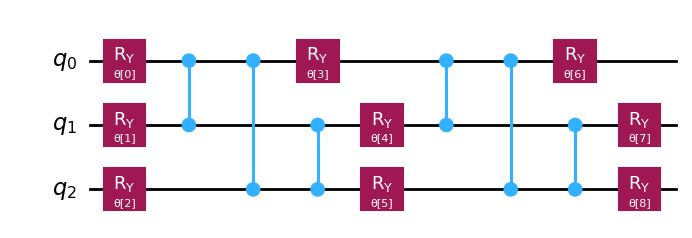
\includegraphics[width=0.45\textwidth]{400/anssatz.png}
        \caption{The ansatz generated for the max-cut example}
        \label{fig:enter-labela}
    \end{figure}
\end{frame}


\begin{frame}{VQE Results}{Single Run}
\begin{itemize}
    \item First discussed is a single run of VQE. 
    \item Included below is a plot of the cost function over the number of iterations. 
    \item Also included is a random sample of the final parameters applied to ansatz, and measured (1000 shots). This should produce the eigenvector associated with the found minimum eigenvalue.
\end{itemize}
\begin{tabular}{c|c|c}
   \# & State & Prob \\
   \hline
   3  & $|011\rangle$ & .405 \\
   4 & $|100 \rangle$ & .595
\end{tabular}

\begin{figure}
    \vspace{-12 mm}
    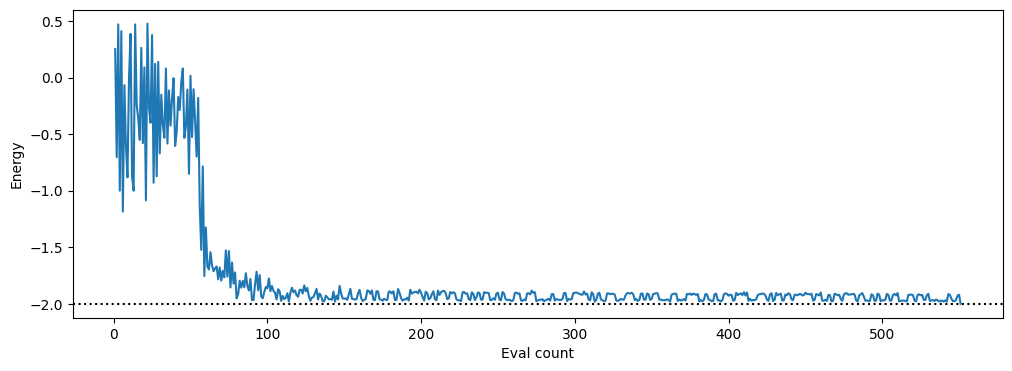
\includegraphics[width=0.75\textwidth]{400/VQE_MC.png}
    \label{fig:enter-label}
\end{figure}

\end{frame}

\begin{frame}{VQE Results}{Multiple Runs}
    \begin{itemize}
        \item Instead, I now conducted multiples run of the same VQE setup in an attempt to determine whether the ansatz was preferring one of the two basis states
        \item Below is the results from 1000 independently run experiments. The probability of each basis state is averaged over every run. Thus, this the expected probability for an additional run of VQE

        \begin{center}
            \begin{tabular}{c|c}
               State  & Expected Probability \\
               \hline
                $|000\rangle$ & 0.000024 \\
                $|001\rangle$ & 0.000156 \\
                $|010\rangle$ & 0.000287 \\
                $|011\rangle$ & 0.505488 \\
                $|100\rangle$ & 0.493707 \\
                $|101\rangle$ & 0.000143 \\
                $|110\rangle$ & 0.000140 \\
                $|111\rangle$ & 0.000055 \\
            \end{tabular}
        \end{center}
        
    \end{itemize}
\end{frame}


\begin{frame}{Qiskit Estimators}
    \begin{enumerate}
        \item Store the Ansatz and Hamiltonian Operator. Copy each a \textbf{\# of Pauli strings} number of times
        \item As many jobs are fed to the backend at once as possible. Once the overall expectation value is completed from the individual Pauli strings, it is fed to the optimizer
        \item From the result, the optimizer guesses a new set of parameters, and the process is repeated.
        \item The stopping mechanism depends on the optimizer. Typically, a convergence threshold detecting changes in the value, or a gradient approximation is used.
        \item SPSA using gradient approximation, and stops when the estimated change in value is small enough
    \end{enumerate}
\end{frame}


\begin{frame}{Hamiltonian Decomposition: 2x2 Naive Approach}
    \begin{itemize}
        \item We will now discuss methods for decomposition of Hamiltonians into Pauli Strings.
        \item We will start with a naive simple method which assumes that imaginary constants are allowed. We will also discuss a more practical approach
        \item Assume the Pauli Matrices are formatted in the following way:
    \end{itemize}
    \[
    \frac{\Identity + \PauliZ}{2} = \begin{bmatrix}
    1 & 0 \\
    0 & 0 \\
    \end{bmatrix} \quad
    \frac{\Identity - \PauliZ}{2} = \begin{bmatrix}
    0 & 0 \\
    0 & 1 \\
    \end{bmatrix} \quad
    \frac{\PauliX + \NiceI \PauliY}{2} = \begin{bmatrix}
    0 & 1 \\
    0 & 0 \\
    \end{bmatrix} \quad
    \frac{\PauliX - \NiceI \PauliY}{2} = \begin{bmatrix}
    0 & 0 \\
    1 & 0 \\
    \end{bmatrix}
    \]    
\end{frame}

\begin{frame}{Naive Approach Continued}
\begin{itemize}
    \item It is easily to see from these combinations that the 4 created gates will span all 2x2 hermitian matrices. 
    \item Considering the tensor products of these gates, we could also span higher dimensional systems
    \item This is one possible way to represent a Hamiltonian in the Pauli basis, but given our understanding of VQE, complex coefficients don't make much sense
    \item The next considered approach is guaranteed to produce real coefficients
    
\end{itemize}
    
\end{frame}

\begin{frame}{The Trace of Pauli Matrices}
\begin{itemize}
    \item In linear algebra, the trace is the sum of the components on the main diagonal of a matrix
    \item Let us consider all combinations of the \PauliX \hspace{1mm} to illustrate the trace behavior
    \[ tr(\PauliX \PauliX) = tr(\Identity) = 2  \quad \quad tr(\PauliX \PauliY) = tr(\begin{bmatrix}
        i & 0 \\
        0 & -i \\
    \end{bmatrix}) = 0\]
    \[ tr(\PauliX \PauliZ) = tr(\begin{bmatrix}
        0 & -1 \\
        1 & 0 \\
    \end{bmatrix}) = 0 \quad \quad tr(\PauliX \Identity) = tr(\PauliX) = 0 \]

    \item Given the expressions for \PauliX, the other Pauli gates can also be confirmed. We arrive at the following generalized relation: $tr(\sigma_i \sigma_j) = 2*\delta_{ij}$
    
\end{itemize}    
\end{frame}

\begin{frame}{Past 1 Qubit}
    \begin{itemize}
        \item Suppose that A and B are two $2^n x 2^n$ gates, no longer 2x2.
        \item Suppose A and B are each represented by Pauli strings. We will attempt to generalize the trace relation to larger Hamiltonians.
    \[Tr(AB) = Tr(\sum_{i \in \{\Identity,\PauliX,\PauliY,\PauliZ\}^{\TensOp n}}^n x_i (\sigma_{i_{1}} \TensOp ... \TensOp \sigma_{i_{n}}) \sum_{j \in \{\Identity,\PauliX,\PauliY,\PauliZ\}^{\TensOp n}}^n y_j (\sigma_{j_{1}} \TensOp ... \TensOp \sigma_{j_{n}}))
    \]

    
    \[= \sum_{i,j \in \{\Identity,\PauliX,\PauliY,\PauliZ\}^{\TensOp n}}^n x_i y_j Tr(\sigma_{i_{1}}\sigma_{j_1} \TensOp ... \TensOp \sigma_{i_{n}}\sigma_{j_n})
    \]

    \[= \sum_{i,j \in \{\Identity,\PauliX,\PauliY,\PauliZ\}^{\TensOp n}}^n x_i y_j \prod_{k=1}^n Tr(\sigma_{i_k} \sigma_{j_k})
    \]
        
    \end{itemize}
    
\end{frame}

\begin{frame}{Past 1 Qubit: Continued}

\[=\sum_{i,j \in \{\Identity,\PauliX,\PauliY,\PauliZ\}^{\TensOp n}}^n x_i y_j ( 2^n \prod_{k=1}^n \delta_{i_k}^{j^k})
\]

\[= 2^n  \sum_{i,j \in \{\Identity,\PauliX,\PauliY,\PauliZ\}^{\TensOp n}}^n x_i y_j \delta_j^i
\]

\[= 2^n \sum_{i \in \{\Identity,\PauliX,\PauliY,\PauliZ\}^{\TensOp n}}^n x_i y_i
\]    
\end{frame}

\begin{frame}{A Decomposition Formulation}
\begin{itemize}
    \item Let $\Tilde{\sigma_k}$ be a given Pauli string for a n dimensional system. We will still assume our Hamiltonian is composed of the sum of Pauli strings
    \item For example, $\Tilde{\sigma_k}$ can take 4 values for 1 qubit. It will have $4^n$ possible values

    
    Assume: 
    \vspace{-3mm}
    \[H = \sum_j s_j \Tilde{\sigma_j }
    \]

    \[Tr(\Tilde{\sigma_k} H) = Tr(\Tilde{\sigma_k}\sum_js_j\Tilde{\sigma_j })
    \]

    % \item Property of Trace: $Tr(aA \TensOp bB) = aTr(A) * bTr(B)$

    \item If j = k, $Tr(\Tilde{\sigma_k} s_j \Tilde{\sigma_j}) = 2^n$, else $Tr(\Tilde{\sigma_k} s_j \Tilde{\sigma_j}) = 0$. Thus, 
   
    \[Tr(\Tilde{\sigma_k} H) = 2^n s_k\]

    \[s_k = \frac{Tr(\Tilde{\sigma_k}H)}{2^n}
    \]
    

    
\end{itemize}
    
\end{frame}

\begin{frame}{Testing it out with our Max Cut Example}{n=3}
    \begin{itemize}
        \item The problem then boils down to calculating $Tr(\Tilde{\sigma_k}H)$ efficiently
        \item These calculations scale exponentially. 
        \item Methods exist to create speedup in specific forms of matrices. 
        

        \[Tr((\PauliZ \TensOp \PauliZ \TensOp \Identity)(H)) = 8 \quad \quad s_{ZZI} = 1
        \]
        \[Tr((\PauliZ \TensOp \Identity \TensOp \PauliZ)(H)) = 8 \quad \quad s_{ZZI} = 1
        \]
        \item All other $s_k$ will be zero.
    \end{itemize}
\end{frame}

\begin{frame}{Tensorized Pauli Decomp}{Matrix Splicing}
    \begin{itemize}
        \item Assume we have n=3 8x8 Hamiltonian.
        \item We can break it down into 4 4x4 Hamiltonians.
        \item These 4 Hamiltonians can be broken down into 16 2x2 Hamiltonians
        \item These 16 Hamiltonians can be broken down into 64 1x1 Hamiltonians.
        \item These are our weights since the trace of a 1x1 is its entry. This process is often faster than matrix multiplication, but is still exponential time complexity (Qiskit used to use the prior mentioned example but now uses this)
        \item \textbf{If this process is exponential, how can the whole VQE process be more efficient than classical systems?}
    \end{itemize}
\end{frame}

\begin{frame}{Arthur Example}
    \begin{itemize}
        \item Let's try a weighted Max Cut example
        \item Given, our logic from the last max cut example, we can easily formulate a Hamiltonian over every included edge. Remember, every node gets a Pauli-Z gate when its included in an edge:
        \[H = 3(\PauliZ \TensOp \Identity \TensOp \Identity \TensOp \PauliZ) + 8(\PauliZ \TensOp \Identity \TensOp \PauliZ \TensOp \Identity) + 3(\PauliZ \TensOp \PauliZ \TensOp \Identity \TensOp \Identity) + 6(\Identity \TensOp \PauliZ \TensOp \PauliZ \TensOp \Identity)
        \]
        \begin{figure}[h]
            \centering
            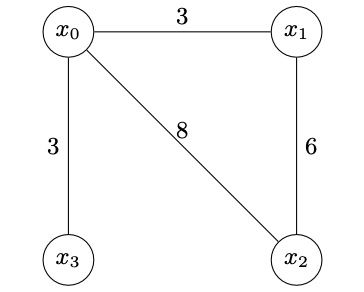
\includegraphics[width=0.3\textwidth]{400/Weighted_Max_Cut.png}
        \end{figure}
        
    \end{itemize}
    
\end{frame}

\begin{frame}{Brute Force of a Weighted Example}
    \begin{itemize}
        \item Let's calculate the expectation value of every computational basis vector on the given Hamiltonian. 
        \item Again, this would not be possible for higher dimensional systems
        
        \centering \begin{tabular}{c|c|c|c}
             $| \psi \rangle$& $E(| \psi \rangle)$ & $| \psi \rangle$ & $E(| \psi \rangle)$ \\
             $|0000\rangle$ & 20 & $|1000\rangle$ & -8 \\
             $|0001\rangle$ & 14 & $|1001\rangle$ & -2 \\
             $|0010\rangle$ & -8 & $|1010\rangle$ & -4 \\
             $|0011\rangle$ & -14 & $|1011\rangle$ & 2 \\
             $|0100\rangle$ & 2 & $|1100\rangle$ & -14 \\
             $|0101\rangle$ & -4 & $|1101\rangle$ & -8 \\
             $|0110\rangle$ & -2 & $|1110\rangle$ & 14 \\
             $|0111\rangle$ & -8 & $|1111\rangle$ & 20 \\
             
        \end{tabular}
        \item 12 ($|1100\rangle$) and 3 ($|0011\rangle$) are maximal cuts of the system
    \end{itemize}
\end{frame}

\begin{frame}{Weighted Example Run on a Simulator}
    \begin{figure}[h]
            \centering
            \includegraphics[width=0.8\textwidth]{400/Screenshot 2024-04-14 at 7.58.37 PM.png}

    \begin{itemize}
        \item The finalized ansatz parameters were once again fed into the ansatz to determine the solution state vector.
        \item The solution produced for this single VQE run was 12
        \item The graph is cleaner due to the COBYLA optimizer, which is threshold-based
    \end{itemize}
    \end{figure}
\end{frame}

\begin{frame}{The H2 Molecule}
    \begin{itemize}
        \item Two Hydrogen atoms, each with one orbital
        \item The orbital can be occupied by two electrons, one spin up and one spin down
        \item Thus, 4 electrons can be present in H2
        \item 4 qubits will be utilized
    \end{itemize}
\end{frame}

\begin{frame}{Chemistry? Oh boy}
    \begin{itemize}
        \item So how would we decompose an atom into a qubit Hamiltonian?
        \item We have an atomic Hamiltonian, although its form is not suitable for qubits
        \[H = -\sum_{i=1}^N{\frac{1}{2}*\nabla_i^2 - \sum_{A=1}^M{\frac{1}{2M_A}\nabla_A^2} - \sum_{i=1}^N{\sum_{A=1}^M{\frac{Z_A}{r_{iA}}}}} + \sum_{j>i}{\frac{1}{r_{ij}}} + \sum_{B>A}{\frac{Z_AZ_B}{R_{AB}}}
        \]
        \quad \quad Electronic KE \quad \quad Nuclear KE \quad \quad e-N C \quad \quad \quad e-e C \quad \quad  N-N C 
        \item C-Coulomb. Born-Oppenheimer Approx says Nuclei are frozen compared to electrons.
        \item Thus, Nuclear KE is about zero and N-N Coulomb is a constant shift.
        \item This allows us to simplify the Hamiltonian further.
    \end{itemize}
\end{frame}
\begin{frame}{Second Quantization Form}
    \begin{itemize}
        \item \textbf{Forms for expressing multi particle states}
        \item First Quantization Form: $|\psi_{tot}\rangle = |\psi_1\rangle\TensOp|\psi_2\rangle\TensOp...\TensOp|\psi_n\rangle$ (3n qubits)
        \item Need to add more about second quantization 
    \end{itemize}
\end{frame}


\begin{frame}{Hamiltonian Decomp}
    \begin{itemize}
        \item 1 body term $a_i^+a_j^-$ is occupation if $i=j$ and electron swap from j to i if $i\neq j$
        \item 2 body term: $a_i^+a_j^+a_k^-a_m^-$
    \end{itemize}
    \begin{equation}
        H_e = -\sum_{i,j}{\frac{1}{2}\langle i | \nabla_i^2 | j \rangle a_i^+a_j^-} + \sum_{i,j}{\langle i | \frac{Z_A}{r_{iA}}| j \rangle a_i^+a_j^- } + \sum_{i,j,k,m}{\langle i,j | \frac{1}{r_{i,j}}| k,m \rangle a_i^+a_j^+a_k^-a_m^-}
    \end{equation}

    \begin{equation}
        H_e = \sum_{p,q}h_{pq}a_p^+a_q^- + \frac{1}{2} \sum_{p,q,r,s}{h_{pqrs}a_p^+a_q^+a_ra_s}
    \end{equation}

    \begin{itemize}
        \item $h_{pq}$ is one body integral $h_{pqrs}$ is twobody integral
        \item Both are found using quantum chemistry calculations
        \item For now, let's assume we've solved out for both computationally. I'll provide the expressions for completeness
    \end{itemize}
    
\end{frame}
\begin{frame}{Body Integrals}
\begin{equation}
    h_{pq} = \int \phi_p^*(r)(-\frac{1}{2} \nabla^2 - \sum_A{\frac{Z_A}{|r-R_A|})\phi_q(r)dr}
\end{equation}

\begin{equation}
    h_{pqrs} = \int{\int{\phi_p^*(r_1)}\phi_q(r_1)\frac{1}{|r_1-r_2|}\phi_r^*(r_2)\phi_s(r_2)dr_1dr_2}
\end{equation}

\begin{itemize}
    \item $\phi_i$ are molecular orbitals
    \item $r_i$ is the coordinate of the i'th electron
    \item $Z_A$ is the charge of the nucleus and $R_A$ is the position of the nucleus
    \item Summing over A is over all Nuclei in Nucleus
    \item Found computationally through classical modeling, but can be found efficiently \textbf{ADD MORE HERE}
\end{itemize}
    
\end{frame}
\begin{frame}{Interpreting the Operators}
\begin{figure}
    \centering
    \includegraphics[width=0.9\textwidth]{400/Screenshot 2024-04-17 at 6.26.40 PM.png}
\end{figure}
    
\end{frame}

\begin{frame}{Body Values for H2}
    \begin{itemize}
        \item The single and two body constants were calculated for an H2 molecule separated by .8 Angstrom. Constant shift: 0.6615
        \item $h_{00}$ = $h_{11}= -1.2178$
        \item $h_{22} = h_{33} = -0.5096$
        \item $h_{0022} = h_{0132} = h_{0202} = h_{0312} = h_{1023} = h_{1133} = h_{1203} = h_{1313} = h_{2020} = h_{2130} = h_{2200} = h_{2310} = h_{3021} = h_{3131} = h_{3201} = h_{3113} = 0.0923$
        \item $h_{0220} = h_{0330} h_{1221} = h_{1331} = h_{2002} = h_{2112} = h_{3003} = h_{3113} = 0.3267$
        \item $h_{2332} = h_{2222} = h_{3223} = h_{3333} = 0.3434$
    \end{itemize}
\end{frame}



\begin{frame}{Anti commutators}
    \begin{itemize}
        \item So why are qubits different from electrons?
        \item Qubits are distinguishable (they commute): $|\psi_{tot}\rangle = |x_1\rangle_1 |x_2\rangle_2$
        \item $e^-$ are indistinguishable (they anti-commute) $|\psi_{tot}\rangle = (|x_1\rangle_1 |x_2\rangle_2-|x_2\rangle_1|x_1\rangle_2)$
        \item For flipping $e_1$ to $e_2$, $|\psi_{tot}\rangle=-|\psi_{tot}\rangle$
        \item Commutator: $[A,B]=AB-BA$
        \item Anti-Commutator: $[A,B]_{+} = AB+BA$
        \item $[A,B]_{+}=0$ or $AB=-BA$
        \item Switching two particles will add a phase of (-1) to the system
        \begin{equation}
            [a_p^-,a_q^-]_+=[a_p^+,a_q^+]_+ = 0
        \end{equation}
        \begin{equation}
            [a_p^-,a_q^+]_+ = \delta_{pq}
        \end{equation}
    \end{itemize}
\end{frame}




\begin{frame}{Fock Space}
    \begin{itemize}
        \item Assume we have M fermions (electrons) in N orbitals. 
        \item Let's form a bit string where each orbital is given a slot in our bit string. If the electron is there, we input 1, if it is empty, 0.
        \item There are $\binom{N}{M}$ ways to fill in M electrons.
        \item$\sum_{i=0}^N{\binom{N}{i}} = 2^N$. There are $2^N$ ways to fill N electrons or less in N orbitals.
        \item Assume each bit string representing a permutation is a column. This $2^N$ square matrix is the Fock Space for Fermions
    \end{itemize}
\end{frame}
\begin{frame}{Fock Space N=3}
    \centering \begin{tabular}{c|c|c|c|c|c|c|c}
         $|000\rangle$ & $|001\rangle$ & $|010\rangle$ & $|100\rangle$ & $|011\rangle$ & $|101\rangle$ & $|110\rangle$ & $|111\rangle$\\
         1 & 0 & 0 & 0 & 0 & 0 & 0 & 0 \\
         0 & 1 & 0 & 0 & 0 & 0 & 0 & 0 \\
         0 & 0 & 1 & 0 & 0 & 0 & 0 & 0 \\
         0 & 0 & 0 & 0 & 1 & 0 & 0 & 0 \\
         0 & 0 & 0 & 1 & 0 & 0 & 0 & 0 \\
         0 & 0 & 0 & 0 & 0 & 1 & 0 & 0 \\
         0 & 0 & 0 & 0 & 0 & 0 & 1 & 0 \\
         0 & 0 & 0 & 0 & 0 & 0 & 0 & 1 \\
    \end{tabular}
    \begin{itemize}
        \item This is known as the occupation number basis for n=3
    \end{itemize}
\end{frame}

\begin{frame}{Ladder Operators}
\begin{itemize}
    \item In QM, Ladder operators allow us to climb between successive states.
    \item A raising operator takes you up a state. The lowering takes you down. 
    \item On one qubit, they would have the following effect
    \item $a^+|0\rangle = |1\rangle$ \quad $a^+|1\rangle = 0$ \quad \quad \quad \quad $a^- |0\rangle = 0$ \quad $a^- |1\rangle = |0\rangle$
    \item We can thus form the 1 qubit ladder operators:
    \[\sigma^+ = \begin{bmatrix}
        0 & 0 \\
        1 & 0 \\
    \end{bmatrix}
    \] \quad \quad \[\sigma^- = \begin{bmatrix}
        0 & 1 \\
        0 & 0 \\
    \end{bmatrix}
    \]
\end{itemize}

\end{frame}

\begin{frame}{Generalized Ladder Operators}
    \begin{equation}
        a^+ |f_{n-1}...f_{j+1}\, 0\, f_{j-1}...f_0\rangle = (-1)^{\sum_{s=0}^{j-1}{f_s}}|f_{n-1}...f_{j+1}\, 1 \, f_{j-1}...f_0\rangle
    \end{equation}
    \begin{equation}
        a^+ |f_{n-1}...f_{j+1}\, 1 \, f_{j-1}...f_0\rangle = 0
    \end{equation}
    \begin{equation}
        a^- |f_{n-1}...f_{j+1}\, 1\, f_{j-1}...f_0\rangle = (-1)^{\sum_{s=0}^{j-1}{f_s}}|f_{n-1}...f_{j+1}\, 0 \, f_{j-1}...f_0\rangle
    \end{equation}
    \begin{equation}
            a^- |f_{n-1}...f_{j+1}\, 0 \, f_{j-1}...f_0\rangle = 0
    \end{equation}

    \begin{itemize}
        \item Suppose: $a_j^+ = \PauliZ^{\TensOp j}\TensOp \sigma^+ \TensOp \Identity^{n-j-1}$
        \item $a_j^- = \PauliZ^{\TensOp j}\TensOp \sigma^- \TensOp \Identity^{n-j-1}$
    \end{itemize}
\end{frame}

\begin{frame}{Proving Multi-Qubit Ladder Operators}{Raising Operator}
    \begin{itemize}
        \item Assume our state is currently $|10\rangle$ and we wish to excite the second electron
        \item We would apply $a_1^+ = (\PauliZ \TensOp \sigma^+)$

        \[(\PauliZ \TensOp \sigma^+ )|10\rangle = - |11\rangle\]

        \item Now assume we are in $|11\rangle$

        \[(\PauliZ \TensOp \sigma^+ )|11\rangle = 0\]
        \item Similarly, for the lowering operator: 

        \[(\PauliZ \TensOp \sigma^-) |11\rangle = -|10\rangle\]

        \[(\PauliZ \TensOp \sigma^-) |10\rangle = 0\]
    \end{itemize}
\end{frame}

\begin{frame}{Closed Form Expression for Ladder Operators}
    \begin{equation}
        a_j^+ = \PauliZ^{\TensOp j}\TensOp \sigma^+ \TensOp \Identity^{n-j-1}
    \end{equation}
    \begin{equation}
        a_j^- = \PauliZ^{\TensOp j}\TensOp \sigma^- \TensOp \Identity^{n-j-1}
    \end{equation}
\end{frame}

\begin{frame}{Ansatz Details}
    
\end{frame}






